\chapter{Estimation of System Matrices}

\section{Introduction}
This document will describe the strategy for obtaining the system matrices(${\phi}_L$ and ${\phi}_R$) of the mask produced by the SLM in front of the sensor. The experimental setup consists of an LCD screen placed at 20 cm from the SLM-sensor setup. The LCD will be used to project objects and patterns in front of the sensor. The experimental setup is shown in Figure \ref{fig:experiment_lcd}.
Initially, I tried projecting a complete blank white pattern on the LCD but the sensor recorded a blank image. I expected that the sensor would give me an image that would represent the mask itself. I tried to move the mask-sensor closer to the LCD as I thought that it might be due to not enough light reaching the sensor, but it also made no difference.The reasoning behind this is due to vignetting of light by the pattern. I tried projecting an horizontal dividable pattern on the LCD to see if there is any variation in intensity across the sensor, but there was no difference in intensity across the output image. Then, I decided to project a circular pattern, to see if there is any difference in the readings from the CMOS sensor. I projected two patterns, a white circle in a black background and a black circle in a white. On seeing the outputs through the naked eye, I found that there was not much difference. To my surprise, on subtracting the two output images, there were slight patterns seen on the difference image. So, I decided to develop a strategy that would enable me to estimate the system matrices.

\begin{figure}[h]
\centering
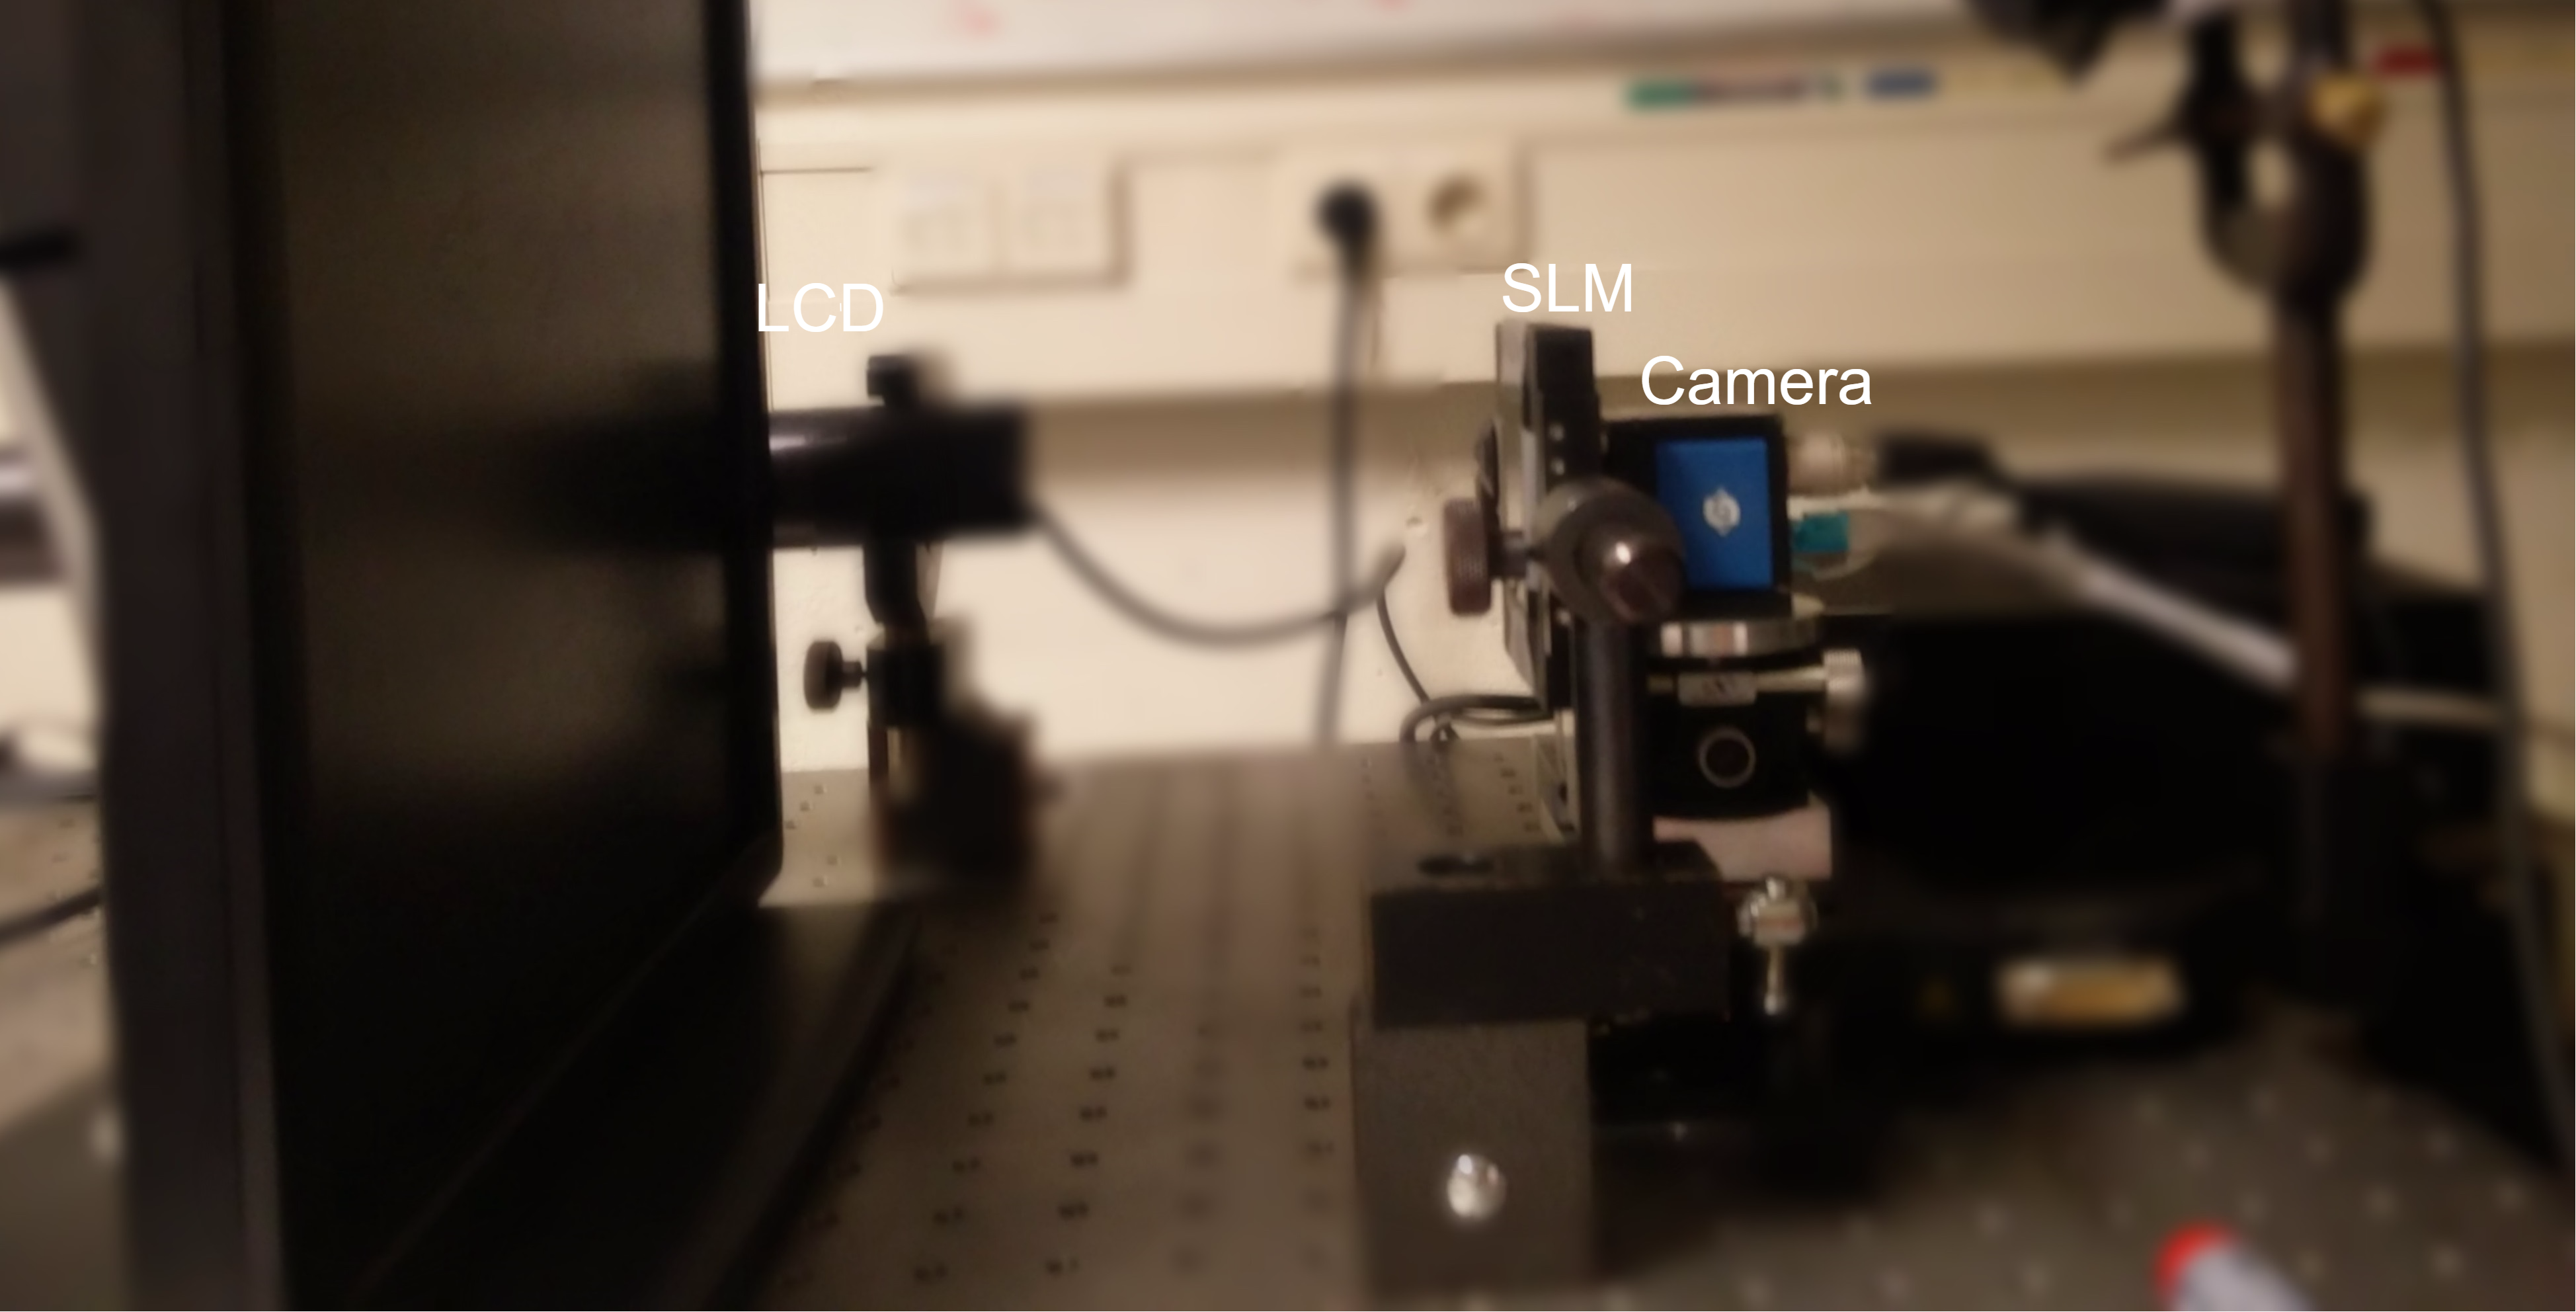
\includegraphics[width = 0.75\linewidth]{pics/experiment_lcd}
\caption{Setup for Intial Experiments}
\label{fig:experiment_lcd}
\end{figure}

\section{Strategy}
The following precautions are taken to make sure that we can accurately estimate the system matrices.
\begin{itemize}
\item Even thought the sensor is measuring only one portion of the LCD, during the initial experiments, it was observed that the entire LCD is contributing to the image on the sensor. There was a noticeable variation in intensity when I tried to block the light from the LCD portion not facing the sensor. So, I decided to block the light from the surrounding pattern using black cardboards.
\item I use the same idea from \cite{Flatcam} to determine the system matrices. If the scene in front of the mask-sensor arrangement is separable, then the sensor output must also be separable. If the scene is of the form $ab^T$, then the image formed on the sensor will be of the form:

\begin{equation}
I = (M_xa)(M_yb)^T
\end{equation}
If the scene can be represented in the form of $a1^T$, then the scene formed on the sensor will be,
\begin{equation}
Y = (M_xa)(M_y)^T
\label{eq:separ_eq}
\end{equation}
On performing singular value decomposition on the scene and approximating the rank-1 matrix(represented in the form $Y_k = u_k v^T$) from the output image we must be able to estimate the left system matrix using the equation:
\begin{equation}
M_x = u_ka^{-1}
\end{equation}
\item For the right system matrix, we can use patterns in the form of $1a^T$, and estimate $M_y$. In the coming sections, we would look at what kind of pattern can be projected on the screen to accurately estimate the right and left system matrices. 
\end{itemize}
\subsection{Identity Basis}
In order to estimate the system matrices, we can use the idea described previously, but we need to decide what patterns need to be used and hoe we can mathematically simulate and verify our idea. We use a invertible base matrix to generate different patterns that can be projected on the LCD screen. The basis matrix pattern can any pattern that would be optically feasible and invertible.
\begin{equation}
B = \begin{bmatrix} 
    b_{11} & b_{12} & \dots & b_{1n}\\
    \vdots & \vdots & \ddots &\vdots \\
    b_{n1} &  b_{n2} & \dots   & b_{nn} 
    \end{bmatrix}_{n\times n}
    \label{eq:basis_matr}
\end{equation}
For estimating the left system matrix we need to extract the columns from the basis matrix that we use and multiply it with a row vector of 1s as shown by equation \label{eq:pattern}
\begin{equation}
1_{row} = \begin{bmatrix} 
    1 & 1 & \dots &1\\

    \end{bmatrix}_{1\times n}
    \label{eq:one_row}
\end{equation}

\begin{equation}
b_{i} = \begin{bmatrix} 
    b_{i1} \\
    b_{i2} \\
	\vdots\\
    b_{in}
    \end{bmatrix}_{n\times 1}
    \label{eq:one_row}
\end{equation}


\begin{equation}
pattern_{i} = \begin{bmatrix} 
    b_{i1} \\
    b_{i2} \\
	\vdots\\
    b_{in}
    \end{bmatrix}_{n\times 1} *
    \begin{bmatrix} 
    1 & 1 & \dots &1\\

    \end{bmatrix}_{1\times n}
  \label{eq:pattern}
\end{equation}

The image produced by $pattern_i$ on the sensor can be decomposed into $u_iv^T$ using the rank-1 estimation obtained from singular value decomposition(SVD). We need to accumulate the sensor output from each $b_i$ multiplied by the row-one vector and find the corresponding $u_i$. These $u_i$ need to be put together to form an $n*n$ matrix. The accumulated $u_i$ values correspond to the left system matrix combined with the basis matrix $B$. We can then invert it to obtain the actual system matrix as shown in equation \ref{eq:left_u}.
\begin{equation}
M_x = \begin{bmatrix} 
    u_{1} & \dots & u_i &  \dots & u_n \\
  
    \end{bmatrix}_{n\times n} * B^{-1}
    \label{eq:left_u}
\end{equation}
Similarly, two obtain the right system matrix using patterns obtained from multiplying the rows from the basis matrix and columns of 1s as illustrated by equation \ref{eq:pattern_col}. The accumulated $v_i$ obtained from singular value decomposition can be inverted using the inverse of the basis matrix as done for the left system matrix. The procedure for obtaining the system matrices is illustrated in Figure \ref{fig:sys_est}.
\begin{equation}
pattern_{j} = \begin{bmatrix} 
    b_{j1} & b_{j2} & \dots &b_{jn}\\
    \end{bmatrix}_{1\times n} *
    \begin{bmatrix} 
    1\\
	1\\
    \vdots\\
    1
    \end{bmatrix}_{n\times 1}
  \label{eq:pattern_col}
\end{equation}

\begin{figure}[h]
\centering
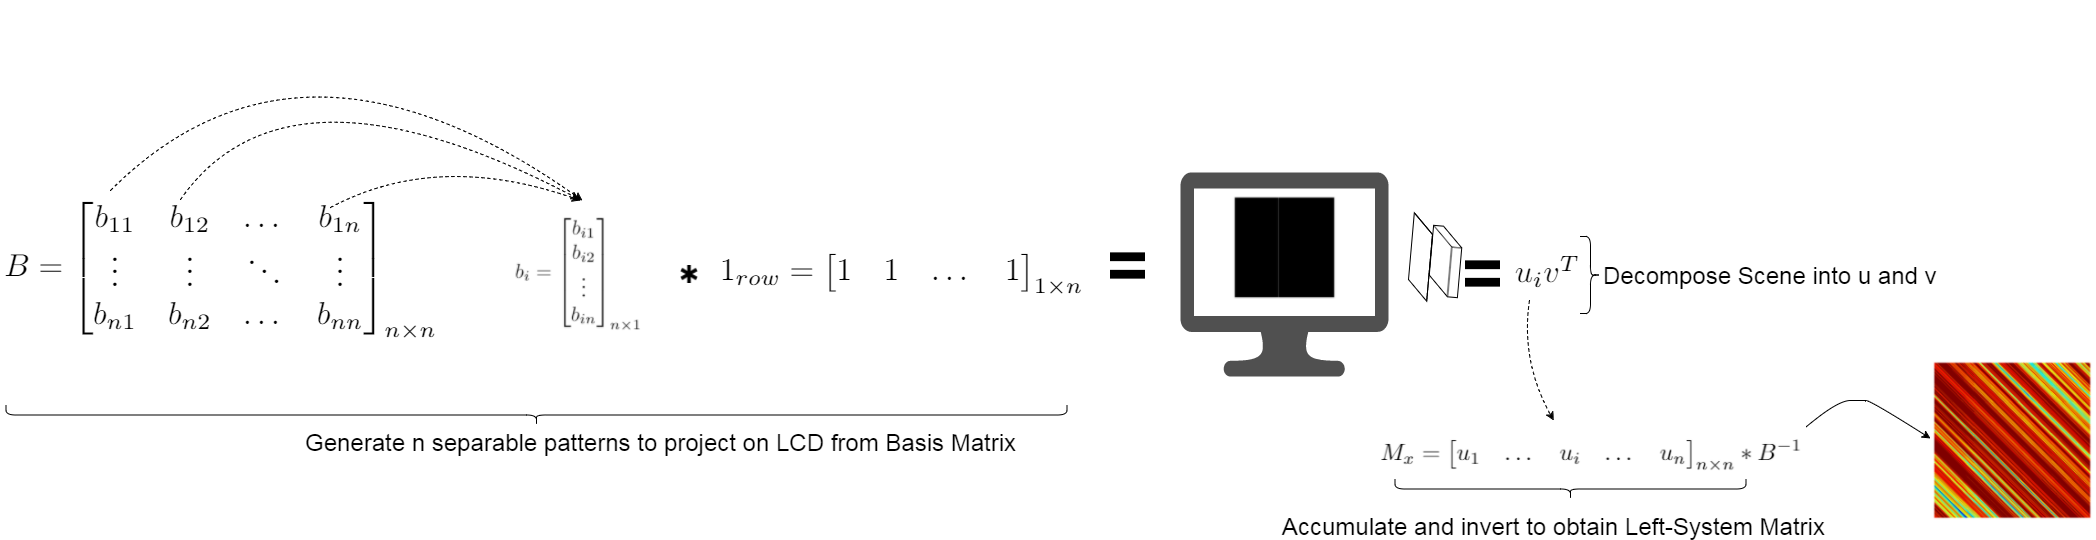
\includegraphics[width = \linewidth]{pics/system_matrix_estimation.png}
\caption{Procedure for obtaining the left system matrix}
\label{fig:sys_est}
\end{figure}
The simplest basis matrix that could be inverted is the identity matrix. The patterns produced by the identity matrix will be a shifting row of ones(white) in a black background for the left system matrix and a shifting column of one in a black background for the right system matrix. This is shown in Figure \ref{fig:pattern_identity}.

\begin{figure}[h]
\centering

\includegraphics[width = \linewidth]{pics/identity_left_right.png}
\caption{Pattern on LCD that would be generated with left and right system matrix}
\label{fig:pattern_identity}
\end{figure}
This entire procedure was simulated on MATLAB like in the previous section and reconstructions obtained using the procedure is compared. The reconstructions obtained by simulating the LCD patterns and obtaining the system matrix is shown in Figure \ref{fig:rec_id}. It can be seen from the figure that the reconstruction obtained using the procedure mentioned leads to a poorer reconstruction than the one which we obtained using the known diffracted mask pattern.
\begin{figure}[h]
\centering
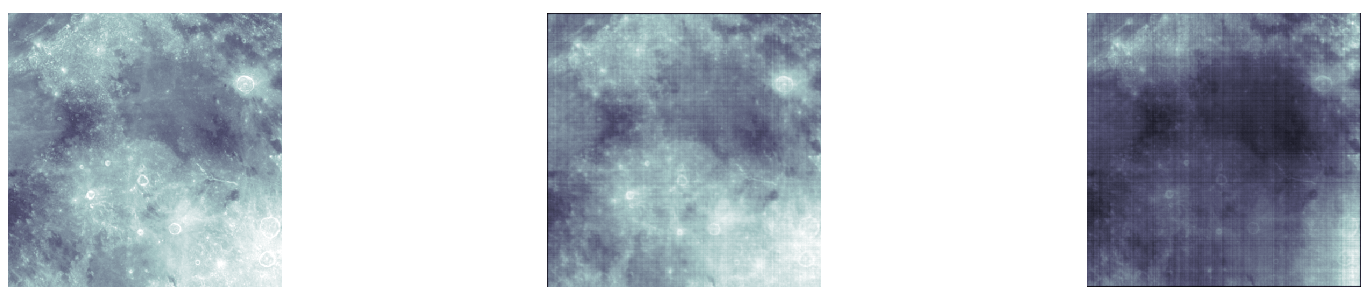
\includegraphics[width = \linewidth]{pics/id_reconst.png}
\caption{This figure shows the differences in reconstruction. The figure on the left most corner is the original object, the middle image represents the inversion obtained using the known diffracted mask pattern, and the right image indicates the reconstruction obtained using simulated LCD patterns and obtaining system matrix. It can bee seen that there is an extreme loss of detail when we try to manually obtain the system matrix using the procedure stated.}
\label{fig:rec_id}
\end{figure}
The system matrix obtained by using the procedure explained above does not provide accurate reconstructions. This problem was traced to the accuracy of the \texttt{svd} function in MATLAB which is used for computing the left and the right vectors when analyzing the scene separability. One more issue with using the identity matrix is that this basis matrix generates a very less amount of light. Projecting these patterns on the LCD did not provide any noticeable change on the sensor in the experimental setup. So, it was decided to use some other basis matrix for estimating the system matrices. The inaccuracy in estimating the left and right vectors is resolved mathematically as explained in the next section. 
\subsection{Hadamard Basis}
In this section we will first discuss an alternative way of obtaining the left and the right system vectors instead of using \texttt{svd} function in MATLAB as it does not provide accurate estimation of a separable scene. Consider that a scene of the form $a1^T$ is imaged by the sensor with the mask. The image on the sensor can be written in the form given by equation \ref{eq:separ_eq}. It can be re-written as shown in equation \ref{eq:no_svd_1}.

\begin{equation}
Y(x,y) = \phi_1(x)\phi_2(y)
\label{eq:no_svd_1}
\end{equation}
The term $\phi_1(X)$ and $\phi_2(Y)$ represent $(M_xa)$ and $(M_y)$ of equation \ref{eq:separ_eq}respectively. The integral of equation \ref{eq:no_svd_1} can be represented by equation \ref{eq:no_svd_2}. When we project a scene of the form $a1^T$, equation \ref{eq:no_svd_2} can be re-written as equation \ref{eq:no_svd_3} as a constant 1 vector is the right vector that is used to generate the pattern.
\begin{equation}
\int Y(x,y) \propto \phi_1(x)\int \phi_2(y)dy
\label{eq:no_svd_2}
\end{equation}
\begin{equation}
\int Y(x,y) \propto \phi_1(x) k
\label{eq:no_svd_3}
\end{equation}
When we sum over the sensor output image in the y-direction while projecting  patterns of the  form $a1^T$, we will be only left with the left system matrix multiplied by a constant. Similarly, when we sum over the sensor output image in the x-direction while projecting  patterns of the  form $1a^T$, we will be only left with the right system matrix multiplied by a constant. This also reduces the computational load instead instead of using MATLAB function \texttt{svd} which is highly computationally intensive. Since, we solved the problem of estimating the left and right system matrices by using a simple summation, let us now focus on using a better basis matrix for estimating the system matrices. 

The identity matrix provides a very less amount of light since it produces only one row of emitting light. So, I decided to test some striped separable patterns and see if we are able to receive any response on the sensor. It was observed that striped patterns are able to produce some siginificant sensor response on estimating the left and right system matrix using SVD. So, I decided to look for matrices that can produce striped patterns on the screen. 

\begin{figure}[h]
\centering
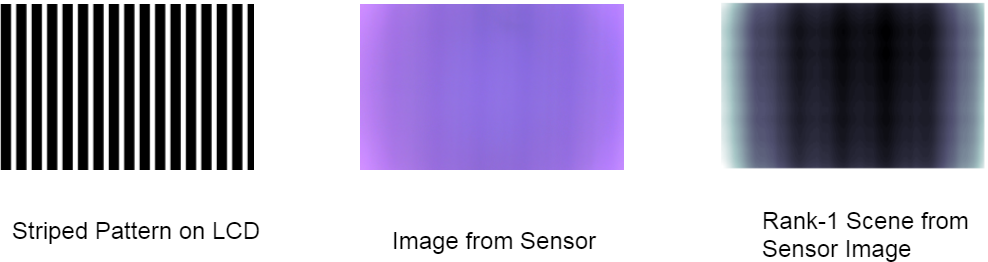
\includegraphics[width = \linewidth]{pics/Striped_Pattern_Response.png}
\caption{This figure indicates the response of the sensor. The right most image is put on the LCD screen. The middle portion indicates the output image from the sensor. The third indicates the rank-1 estimate of the scene obtained using SVD}
\label{fig:str_response}
\end{figure}

In order to accurately estimate the system matrices, we need to project multiple striped patterns. 
We want a matrix that has binary values(1s and 0s) so that we can translate them into color and then work on reconstruction of it. One such pattern is a hadamard pattern which is widely used in compressed image sensing\cite{hadamard}\cite{Flatcam}. This basis matrix is also used in previous studies is the hadamard matrix $H$ whose inverse is of the form given by equation \ref{eq:hadamard_inverse}. The size of the hadamard matrix $n$ is always in the powers of 2.

\begin{equation}
H^{-1} = \frac{1}{n} H^T
\label{eq:hadamard_inverse}
\end{equation}
However, one disadvantage of hadamard matrix is that it has negative one values which is optically not feasible. However, we can follow some mathematical tricks to make it optically feasible. Consider a $2 \times 2$ hadamard matrix shown in equation \ref{eq:hadamard_1}. Let us take the keep the matrix and also take the negative of the matrix.
\begin{equation}
H_2 = \begin{bmatrix} 
       1 & 1 \\
	   1 & -1 \\
    \end{bmatrix}
    \label{eq:hadamard_1}
\end{equation}

\begin{equation}
H_2^+ = \begin{bmatrix} 
       1 & 1 \\
	   1 & -1 \\
    \end{bmatrix}
   \hspace{1cm}
   H_2^- = \begin{bmatrix} 
       -1 & -1 \\
	   -1 & 1 \\
    \end{bmatrix}
    \label{eq:hadamard_2}
\end{equation}
In order to make the mask optically feasible, let us set the negative entries of equation \ref{eq:hadamard_2} to zero.

\begin{equation}
H_2^+ = \begin{bmatrix} 
       1 & 1 \\
	   1 & 0 \\
    \end{bmatrix}
   \hspace{1cm}
   H_2^- = \begin{bmatrix} 
       0 & 0 \\
	   0 & 1 \\
    \end{bmatrix}
    \label{eq:hadamard_3}
\end{equation}
We can see from equation \ref{eq:hadamard_3} that 
\begin{equation}
H_2 = H_2^+ - H_2^-1
\label{eq:hadamard_4}
\end{equation}

By projecting binary patterns of the form given by equation \ref{eq:hadamard_3}, we can make an optically realizable hadamard pattern. However, a disadvantage is that we need to project two kinds of patterns(one for $H^+$ and one for $H^-$) and subtract the sensor images to get the reading for the original hadamard pattern. An example of vertical and horizontal hadamard patterns is shown in Figure \ref{fig:hadamrd_ex}. 

\begin{figure}[h]
\centering

\includegraphics[width = \linewidth]{pics/hadamard_ex.png}
\caption{An example of vertical and horizontal hadamard pattern($H^+$) that can be used for system matrix estimation. Note that the same procedure as mentioned previously holds. Only an additional pattern needs to be incorporated to make the hadamard pattern optically feasible }
\label{fig:hadamrd_ex}
\end{figure}
An example of reconstruction using the hadamrd patterns is shown in Figure \ref{fig:hadamrd_rec}. It can be seen from Figure \ref{fig:hadamrd_rec} that estimating the system matrix manually provides a lot better results and preserves a lot more detail than using the known diffracted mask pattern. 
\begin{figure}[h]
\centering
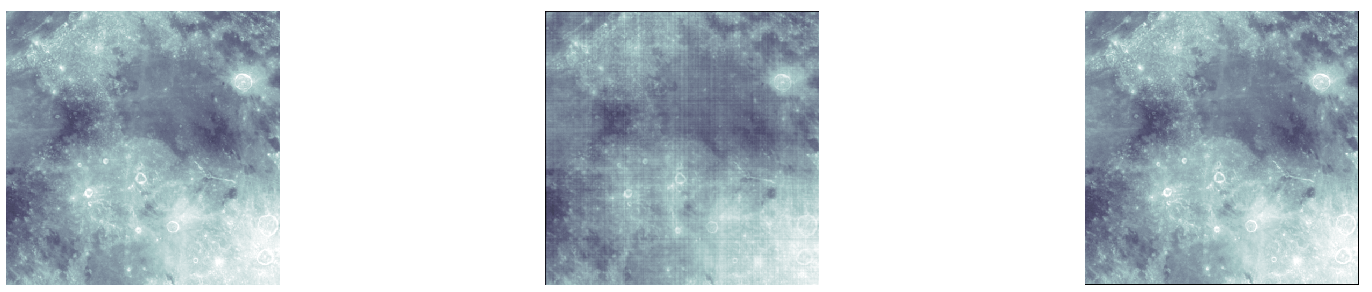
\includegraphics[width = \linewidth]{pics/hadamard_rec.png}
\caption{This figure indicates the reconstructions obtained using the hadamard matrix as the basis matrix and after summing to obtain the separable scene components. The left most image indicates the original object, the middle indicates the reconstruction obtained with known system matrix and the right indicates the reconstruction with the system matrices obtained by projecting hadamard patterns. It can be seen that the effects of noise are no longer visible and the reconstruction is perfect. }
\label{fig:hadamrd_rec}
\end{figure}

We can see that both the basis matrices need measurements from $N\times N$ calibration patterns to reconstruct a $N \times N$ resolution image. We can generate $N \times N$ hadamard patterns and estimate the accurate system matrix that can provide extremely good reconstruction results as seen in the simulation.  